\documentclass[UTF8,fontset=windows]{ctexart}
\usepackage[a4paper,margin=22mm]{geometry}
\usepackage{amsmath,amssymb}
\usepackage{tikz}
\usepackage{booktabs}
\usepackage{enumitem}
\usepackage{xcolor}
\usepackage{float}
\usetikzlibrary{arrows.meta,calc,patterns}

\setlength{\parindent}{0pt}
\setlength{\parskip}{6pt}
\setlist[itemize]{leftmargin=2em,itemsep=2pt,topsep=2pt}

\definecolor{accent}{RGB}{32,92,148}
\definecolor{softblue}{RGB}{224,238,250}
\definecolor{softred}{RGB}{252,230,226}
\definecolor{axisgray}{RGB}{80,80,80}

\newcommand{\diff}{\,\mathrm{d}}

\title{\vspace{-1.5cm}\textbf{清华大学 2001 年《工程力学》期末考试题标准解答}}
\author{考前复习标准答案}
\date{考试日期：2001年1月9日}

\begin{document}
\maketitle
\vspace{-1.0cm}

\section*{一、正弦分布载荷悬臂梁分析题（20分）}

\textbf{1、一悬臂梁长为 $L$，A 端固支，B 端为自由端。梁上受的载荷集度可用一正弦函数表示，如下图所示。试求 B 点的挠度和转角。}

\begin{center}
\begin{tikzpicture}[scale=1.5, >=Stealth]
    % Draw beam
    \draw[ultra thick, accent] (0,0) -- (4,0);
    
    % Support A
    \draw[thick] (0,0.5) -- (0,-0.5);
    \foreach \y in {-0.4,-0.2,0,0.2,0.4} {
        \draw[thin] (0,\y) -- (-0.15,\y+0.1);
    }
    \node at (-0.3,0) {A};
    \node at (4,-0.2) {B};
    
    % Sine load
    \draw[domain=0:4, samples=50, smooth, variable=\x, blue, thick] plot (\x, {0.6*sin(45*\x)});
    \foreach \x in {0.4,0.8,1.2,1.6,2.0,2.4,2.8,3.2,3.6} {
        \draw[->, blue, thin] (\x, {0.6*sin(45*\x)}) -- (\x, 0.05);
    }
    \node[blue] at (2,0.8) {$q(x) = q_0 \sin\left(\frac{\pi x}{L}\right)$};
    
    % Coordinate axes
    \draw[->, gray] (0,0) -- (4.5,0) node[right] {$x$};
    \draw[->, gray] (0,0) -- (0,-1.0) node[below] {$w$ (向下为正)};
    
    % Dimensions
    \draw[<->, gray] (0,-0.4) -- node[fill=white] {$L$} (4,-0.4);
\end{tikzpicture}
\end{center}

\subsubsection*{解答：}

以固定端 A 为坐标原点 $x = 0$，向右为 $x$ 轴正方向；设挠度 $w(x)$ 向下为正。
梁上承受向下的正弦分布载荷，载荷集度方程为：
\[
    q(x) = q_0 \sin\left(\frac{\pi x}{L}\right)
\]
梁的弯曲控制微分方程为：
\[
    EI \frac{\diff^4 w(x)}{\diff x^4} = q(x) = q_0 \sin\left(\frac{\pi x}{L}\right)
\]
对此方程进行逐次积分：

\textbf{1. 积分一次求剪力相关项}
\[
    EI \frac{\diff^3 w(x)}{\diff x^3} = -q_0 \frac{L}{\pi} \cos\left(\frac{\pi x}{L}\right) + C_1
\]
边界条件：在自由端 B ($x = L$) 处，剪力为 0，即：
\[
    V(L) = -EI w'''(L) = 0 \implies -q_0 \frac{L}{\pi} \cos(\pi) + C_1 = 0 \implies q_0 \frac{L}{\pi} + C_1 = 0 \implies C_1 = -q_0 \frac{L}{\pi}
\]
所以：
\[
    EI \frac{\diff^3 w(x)}{\diff x^3} = -q_0 \frac{L}{\pi} \cos\left(\frac{\pi x}{L}\right) - q_0 \frac{L}{\pi}
\]

\textbf{2. 积分两次求弯矩相关项}
\[
    EI \frac{\diff^2 w(x)}{\diff x^2} = -q_0 \left(\frac{L}{\pi}\right)^2 \sin\left(\frac{\pi x}{L}\right) - q_0 \frac{L}{\pi} x + C_2
\]
边界条件：在自由端 B ($x = L$) 处，弯矩为 0，即：
\[
    M(L) = EI w''(L) = 0 \implies -q_0 \left(\frac{L}{\pi}\right)^2 \sin(\pi) - q_0 \frac{L^2}{\pi} + C_2 = 0 \implies C_2 = q_0 \frac{L^2}{\pi}
\]
所以：
\[
    EI \frac{\diff^2 w(x)}{\diff x^2} = -q_0 \left(\frac{L}{\pi}\right)^2 \sin\left(\frac{\pi x}{L}\right) - q_0 \frac{L}{\pi} x + q_0 \frac{L^2}{\pi}
\]

\textbf{3. 积分三次求转角方程}
\[
    EI \frac{\diff w(x)}{\diff x} = q_0 \left(\frac{L}{\pi}\right)^3 \cos\left(\frac{\pi x}{L}\right) - \frac{q_0 L}{2\pi} x^2 + \frac{q_0 L^2}{\pi} x + C_3
\]
边界条件：在固定端 A ($x = 0$) 处，转角为 0，即：
\[
    \theta(0) = \frac{\diff w}{\diff x}(0) = 0 \implies q_0 \left(\frac{L}{\pi}\right)^3 \cos(0) + C_3 = 0 \implies C_3 = -q_0 \left(\frac{L}{\pi}\right)^3
\]
因此，转角方程为：
\[
    EI \theta(x) = q_0 \left(\frac{L}{\pi}\right)^3 \left[\cos\left(\frac{\pi x}{L}\right) - 1\right] - \frac{q_0 L}{2\pi} x^2 + \frac{q_0 L^2}{\pi} x
\]
在自由端 B ($x = L$) 处，B 点的转角为：
\[
    \theta_B = \theta(L) = \frac{q_0}{EI} \left( \left(\frac{L}{\pi}\right)^3 [\cos(\pi) - 1] - \frac{L^3}{2\pi} + \frac{L^3}{\pi} \right) = \frac{q_0 L^3}{\pi EI} \left( \frac{1}{2} - \frac{2}{\pi^2} \right)
\]

\textbf{4. 积分四次求挠度方程}
\[
    EI w(x) = q_0 \left(\frac{L}{\pi}\right)^4 \sin\left(\frac{\pi x}{L}\right) - q_0 \left(\frac{L}{\pi}\right)^3 x - \frac{q_0 L}{6\pi} x^3 + \frac{q_0 L^2}{2\pi} x^2 + C_4
\]
边界条件：在固定端 A ($x = 0$) 处，挠度为 0，即：
\[
    w(0) = 0 \implies C_4 = 0
\]
因此，挠度方程为：
\[
    w(x) = \frac{q_0}{EI} \left( \left(\frac{L}{\pi}\right)^4 \sin\left(\frac{\pi x}{L}\right) - \left(\frac{L}{\pi}\right)^3 x - \frac{L}{6\pi} x^3 + \frac{L^2}{2\pi} x^2 \right)
\]
在自由端 B ($x = L$) 处，B 点的挠度为：
\[
    w_B = w(L) = \frac{q_0}{EI} \left( \left(\frac{L}{\pi}\right)^4 \sin(\pi) - \frac{L^4}{\pi^3} - \frac{L^4}{6\pi} + \frac{L^4}{2\pi} \right) = \frac{q_0 L^4}{\pi EI} \left( \frac{1}{3} - \frac{1}{\pi^2} \right)
\]

\textbf{结论}：B 点的挠度和转角分别为：
\[
    w_B = \frac{q_0 L^4}{\pi EI} \left( \frac{1}{3} - \frac{1}{\pi^2} \right) \quad (\text{向下}), \qquad \theta_B = \frac{q_0 L^3}{\pi EI} \left( \frac{1}{2} - \frac{2}{\pi^2} \right) \quad (\text{顺时针})
\]

\newpage

\section*{二、带拉索工字钢柱稳定性与安全性校核（20分）}

\textbf{2、工字型截面铝梁，下端与地面固定，上端用一钢索来约束其在 $x$ 方向的运动。试确定最大的临界载荷 $P$。若失稳安全因数取 2，校核结构是否安全。（设铝梁的弹性模量 $E=70\text{ GPa}$，屈服极限 $\sigma_s=215\text{ MPa}$，梁的横截面积 $A=7.5 \times 10^{-3}\text{ m}^2$，惯性矩 $I_x=61.3 \times 10^{-6}\text{ m}^4$，$I_y=23.2 \times 10^{-6}\text{ m}^4$，柱长 $L=5\text{ m}$。）}

\begin{center}
\begin{tikzpicture}[scale=1.2, >=Stealth]
    % Column
    \draw[line width=4pt, gray] (0,0) -- (0,4);
    
    % Fixed support at bottom
    \pattern[pattern=north east lines] (-0.5,-0.2) rectangle (0.5,0);
    \draw[thick] (-0.5,0) -- (0.5,0);
    
    % Cable at top
    \draw[dashed, thick, red] (0,4) -- (2,4);
    \fill (2,4) circle (2pt);
    \node[right] at (2,4) {钢索 (限位 $x$ 方向)};
    
    % Load P
    \draw[->, blue, ultra thick] (0,4.8) -- node[left] {$P$} (0,4.1);
    
    % Axes
    \draw[->, black!60] (-1,0) -- (1,0) node[right] {$x$};
    \draw[->, black!60] (0,0) -- (0,5) node[above] {$z$};
    
    % Dimension
    \draw[<->, gray] (-0.5,0) -- node[left] {$L = 5\text{ m}$} (-0.5,4);
\end{tikzpicture}
\end{center}

\subsubsection*{解答：}

该工字型截面立柱的稳定性在两个主平面内约束条件不同，需要分别计算其临界载荷：

\textbf{1. 绕 $x$ 轴弯曲（在 $y-z$ 平面内失稳）}
*   由于顶部钢索仅在 $x$ 方向进行运动约束，因此在 $y$ 方向上，立柱顶部是完全自由的。
*   所以在 $y-z$ 平面内，立柱的边界条件为：底端固定，顶端自由（悬臂柱模式）。
*   对应的长度系数为：$\mu_y = 2.0$。
*   其临界载荷为：
    \[
        P_{\text{cr}, x} = \frac{\pi^2 E I_x}{(\mu_y L)^2} = \frac{\pi^2 \times 70 \times 10^9 \times 61.3 \times 10^{-6}}{(2.0 \times 5)^2} = 42.91 \pi^2\text{ kN} \approx 423.50\text{ kN}
    \]

\textbf{2. 绕 $y$ 轴弯曲（在 $x-z$ 平面内失稳）}
*   在 $x$ 方向，立柱底部固定，顶部有钢索约束，等效为一端固定、另一端铰支。
*   对应的长度系数为：$\mu_x = 0.7$。
*   其临界载荷为：
    \[
        P_{\text{cr}, y} = \frac{\pi^2 E I_y}{(\mu_x L)^2} = \frac{\pi^2 \times 70 \times 10^9 \times 23.2 \times 10^{-6}}{(0.7 \times 5)^2} = \frac{1.624 \times 10^6 \pi^2}{12.25} \approx 132.57 \pi^2\text{ kN} \approx 1308.41\text{ kN}
    \]

\textbf{3. 确定立柱的实际最大临界载荷 $P_{\text{cr}}$}
立柱的临界载荷取决于两者的极小值，即：
\[
    P_{\text{cr}} = \min(P_{\text{cr}, x}, P_{\text{cr}, y}) = 423.50\text{ kN}
\]
立柱将首先在 $y-z$ 平面内发生弯曲失稳。

\textbf{4. 欧拉公式适用性校核}
*   绕 $x$ 轴的回转半径 $i_x$ 为：
    \[
        i_x = \sqrt{\frac{I_x}{A}} = \sqrt{\frac{61.3 \times 10^{-6}}{7.5 \times 10^{-3}}} \approx 0.0904\text{ m} = 90.4\text{ mm}
    \]
*   立柱的最大长细比（柔度）为：
    \[
        \lambda_x = \frac{\mu_y L}{i_x} = \frac{2.0 \times 5}{0.0904} \approx 110.6
    \]
*   铝梁材料的临界柔度 $\lambda_P$ 估计值为（采用屈服极限 $\sigma_s$ 近似比例极限 $\sigma_P$）：
    \[
        \lambda_P = \pi \sqrt{\frac{E}{\sigma_s}} = \pi \sqrt{\frac{70 \times 10^9}{215 \times 10^6}} \approx 56.7
    \]
*   因为 $\lambda_x = 110.6 > \lambda_P = 56.7$，所以立柱属于大柔度压杆，发生的是弹性屈曲，使用欧拉公式计算临界载荷是完全适用且正确的。
*   同时校核其临界应力：
    \[
        \sigma_{\text{cr}} = \frac{P_{\text{cr}}}{A} = \frac{423.50 \times 10^3}{7.5 \times 10^{-3}} \approx 56.47\text{ MPa} < \sigma_s = 215\text{ MPa}
    \]
    未达到屈服极限，更加证明弹性屈曲分析的准确性。

\textbf{5. 安全性校核}
*   许用载荷 $[P]$ 计算为：
    \[
        [P] = \frac{P_{\text{cr}}}{n_{st}} = \frac{423.50}{2} = 211.75\text{ kN}
    \]
*   若实际工作载荷 $P$ 满足 $P \le [P] = 211.75\text{ kN}$，则结构安全；若实际载荷大于 $211.75\text{ kN}$，则结构不安全。

\newpage

\section*{三、中点集中力作用下等应力简支梁设计（20分）}

\textbf{3、要设计一件等应力简支梁如图所示，即要求梁的任意横截面上的最大正应力是材料许用应力 $[\sigma]$。而铰支座附近应该满足韧性材料的切应力准则。设梁的宽度为常数 $b$，长度为 $L$，梁中点受一集中力 $P$ 作用，求梁的高度 $h$ 随梁的轴线位置 $x$ 变化的关系。}

\begin{center}
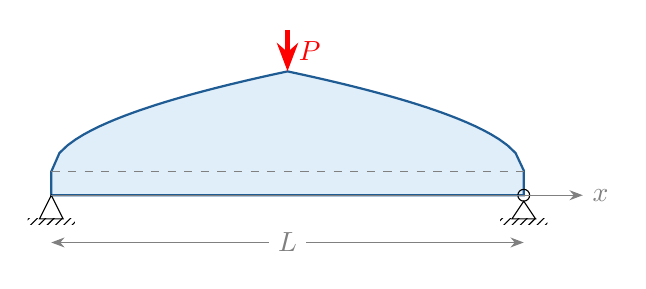
\begin{tikzpicture}[scale=1.5, >=Stealth]
    % Draw equal strength beam (parabolic profile)
    \draw[thick, accent, fill=softblue] (0,-0.2) -- plot[domain=0:2, samples=30] (\x, {0.6*sqrt(\x)}) 
                          -- plot[domain=2:4, samples=30] (\x, {0.6*sqrt(4-\x)}) 
                          -- (4,-0.2) -- cycle;
    
    % Draw axis
    \draw[dashed, gray] (0,0) -- (4,0);
    
    % Supports
    \draw (0,-0.2) -- (-0.1,-0.4) -- (0.1,-0.4) -- cycle;
    \pattern[pattern=north east lines] (-0.2,-0.45) rectangle (0.2,-0.4);
    
    \draw (4,-0.2) circle (0.05);
    \draw (4,-0.25) -- (3.9,-0.4) -- (4.1,-0.4) -- cycle;
    \pattern[pattern=north east lines] (3.8,-0.45) rectangle (4.2,-0.4);
    
    % Load P
    \draw[->, red, ultra thick] (2,1.2) -- node[right] {$P$} (2,0.85);
    
    % Coordinates
    \draw[->, gray] (0,-0.2) -- (4.5,-0.2) node[right] {$x$};
    \draw[<->, gray] (0,-0.6) -- node[fill=white] {$L$} (4,-0.6);
\end{tikzpicture}
\end{center}

\subsubsection*{解答：}

由于简支梁和载荷具有对称性，我们仅需分析左半截面 $x \in [0, L/2]$。

\textbf{1. 确定弯矩方程}
在 $x \in [0, L/2]$ 范围内，梁的支座反力为 $R_A = P/2$，弯矩方程为：
\[
    M(x) = \frac{P}{2} x
\]

\textbf{2. 基于最大正应力条件确定高度 $h(x)$}
对于矩形截面梁（宽为常数 $b$，高度为 $h(x)$），其截面法向抵抗矩为 $W(x) = \frac{1}{6} b h^2(x)$。
截面上的最大正应力必须达到材料的许用应力 $[\sigma]$：
\[
    \sigma_{\max}(x) = \frac{M(x)}{W(x)} = \frac{\frac{P}{2} x}{\frac{1}{6} b h^2(x)} = \frac{3 P x}{b h^2(x)} = [\sigma]
\]
由此求得高度 $h(x)$ 随位置 $x$ 的变化关系为：
\[
    h(x) = \sqrt{\frac{3 P x}{b [\sigma]}}
\]
可见，梁的高度呈抛物线规律变化。在中点 $x = L/2$ 处，高度达到最大值：
\[
    h_{\max} = \sqrt{\frac{3 P L}{2 b [\sigma]}}
\]

\textbf{3. 在铰支座附近应用切应力准则进行校核与修正}
*   在支座附近 $x \to 0$ 时，弯矩 $M(x) \to 0$，若仅按正应力设计，则 $h(0) \to 0$。然而，支座处的剪力不为零，其值为常数 $V(x) = P/2$。
*   矩形截面上最大剪应力发生在中性轴处，其计算公式为：
    \[
        \tau_{\max}(x) = \frac{3 V(x)}{2 A(x)} = \frac{3 P}{4 b h(x)}
    \]
*   根据韧性材料的切应力准则，要求最大切应力不超过许用切应力 $[\tau]$（此处 $[\tau] = 0.5 [\sigma]$ 或 $0.577 [\sigma]$，根据强度理论而定，我们直接用许用切应力符 $[ \tau ]$ 表示）：
    \[
        \tau_{\max}(x) \le [\tau] \implies \frac{3 P}{4 b h(x)} \le [\tau] \implies h(x) \ge h_{\min} = \frac{3 P}{4 b [\tau]}
    \]
*   这说明在支座附近，梁的高度必须保持一个常数 $h_{\min}$，以满足抗剪强度要求。

\textbf{4. 确定转换点位置 $x_0$}
当正应力要求的高度等于剪应力要求的最小高度时，对应的轴线位置为 $x_0$：
\[
    \sqrt{\frac{3 P x_0}{b [\sigma]}} = \frac{3 P}{4 b [\tau]} \implies \frac{3 P x_0}{b [\sigma]} = \frac{9 P^2}{16 b^2 [\tau]^2} \implies x_0 = \frac{3 P [\sigma]}{16 b [\tau]^2}
\]

\textbf{结论}：梁的高度 $h(x)$ 与轴线位置 $x$ 的完整关系（左半跨）为：
\[
    h(x) = \begin{cases}
        \dfrac{3 P}{4 b [\tau]} & x \in \left[ 0, \, \dfrac{3 P [\sigma]}{16 b [\tau]^2} \right] \\[10pt]
        \sqrt{\dfrac{3 P x}{b [\sigma]}} & x \in \left[ \dfrac{3 P [\sigma]}{16 b [\tau]^2}, \, \dfrac{L}{2} \right]
    \end{cases}
\]
右半跨 ($x \in [L/2, L]$) 满足关于跨中对称的分布。

\newpage

\section*{四、受热铝圆柱与钢立柱超静定温度应力分析（20分）}

\textbf{4、在中心铝圆柱 CD 上绕有热电阻丝，通电后将铝圆柱从 $30\text{ °C}$ 加热到 $180\text{ °C}$。在 $30\text{ °C}$ 时，铝圆柱顶端距上面的横梁底面间隙为 $0.7\text{ mm}$。如果设横梁为刚性梁，求两侧钢立柱 AB 和 EF 所受的应力。（铝圆柱截面积为 $375\text{ mm}^2$，钢立柱截面积为 $125\text{ mm}^2$（单侧），铝的弹性模量为 $70\text{ GPa}$，温度膨胀系数为 $23 \times 10^{-6}/\text{°C}$，钢的弹性模量为 $200\text{ GPa}$，钢柱长为 $300\text{ mm}$，铝柱长为 $240\text{ mm}$。）}

\begin{center}
\begin{tikzpicture}[scale=1.2, >=Stealth]
    % Draw rigid top beam
    \draw[ultra thick, fill=gray!30] (-2,2) rectangle (2,2.3);
    \node[above] at (0,2.3) {刚性梁 BF};
    
    % Draw steel columns AB and EF
    \draw[line width=3pt, accent] (-1.5,2) -- (-1.5,-1);
    \draw[line width=3pt, accent] (1.5,2) -- (1.5,-1);
    \node[left] at (-1.5,0.5) {钢柱 AB};
    \node[right] at (1.5,0.5) {钢柱 EF};
    
    % Ground supports for steel columns
    \pattern[pattern=north east lines] (-1.8,-1.2) rectangle (-1.2,-1);
    \draw[thick] (-1.8,-1) -- (-1.2,-1);
    \pattern[pattern=north east lines] (1.2,-1.2) rectangle (1.8,-1);
    \draw[thick] (1.2,-1) -- (1.8,-1);
    
    % Draw aluminum column CD
    \draw[line width=5pt, orange] (0,1.8) -- (0,-1);
    \node[right] at (0,0.4) {铝柱 CD};
    \pattern[pattern=north east lines] (-0.3,-1.2) rectangle (0.3,-1);
    \draw[thick] (-0.3,-1) -- (0.3,-1);
    
    % Gap
    \draw[<->, red, thick] (0,1.8) -- node[fill=white, inner sep=1pt] {$\delta_0$} (0,2.0);
\end{tikzpicture}
\end{center}

\subsubsection*{解答：}

\textbf{1. 自由膨胀变形分析}
若铝圆柱 CD 在不受约束的情况下自由受热膨胀，其温度变形 $\Delta L_{\text{Al}, T}$ 为：
\[
    \Delta L_{\text{Al}, T} = \alpha_{\text{Al}} \cdot \Delta T \cdot L_{\text{Al}}
\]
已知 $\alpha_{\text{Al}} = 23 \times 10^{-6}/\text{°C}$，$\Delta T = 180 - 30 = 150\text{ °C}$，$L_{\text{Al}} = 240\text{ mm}$。代入计算：
\[
    \Delta L_{\text{Al}, T} = 23 \times 10^{-6} \times 150 \times 240 = 0.828\text{ mm}
\]
因为自由膨胀量 $\Delta L_{\text{Al}, T} = 0.828\text{ mm}$ 大于初始间隙 $\delta_0 = 0.7\text{ mm}$，所以铝圆柱的膨胀必定会消除间隙并顶起刚性横梁，使整个系统产生内力（超静定受力状态）。

\textbf{2. 平衡条件分析}
设在平衡状态下，铝圆柱 CD 承受的轴向压紧力为 $F_{\text{Al}}$（以受压为正），两根对称分布的钢立柱承受的轴向拉力均为 $F_{\text{St}}$（以受拉为正）。根据刚性横梁的垂直方向平衡条件：
\[
    \sum F_y = 0 \implies F_{\text{Al}} = 2 F_{\text{St}}
\]

\textbf{3. 变形协调分析}
*   铝圆柱的实际伸长量为温度膨胀减去受压带来的弹性缩短量：
    \[
        \Delta L_{\text{Al}} = \Delta L_{\text{Al}, T} - \frac{F_{\text{Al}} L_{\text{Al}}}{E_{\text{Al}} A_{\text{Al}}}
    \]
*   两侧钢立柱的拉伸量为：
    \[
        \Delta L_{\text{St}} = \frac{F_{\text{St}} L_{\text{St}}}{E_{\text{St}} A_{\text{St}}}
    \]
*   系统整体的变形协调方程为：
    \[
        \Delta L_{\text{Al}} = \delta_0 + \Delta L_{\text{St}}
    \]
    将上式展开：
    \[
        \Delta L_{\text{Al}, T} - \frac{F_{\text{Al}} L_{\text{Al}}}{E_{\text{Al}} A_{\text{Al}}} = \delta_0 + \frac{F_{\text{St}} L_{\text{St}}}{E_{\text{St}} A_{\text{St}}}
    \]

\textbf{4. 联立求解钢立柱的受力}
代入平衡条件 $F_{\text{Al}} = 2 F_{\text{St}}$：
\[
    \Delta L_{\text{Al}, T} - \delta_0 = F_{\text{St}} \left( \frac{2 L_{\text{Al}}}{E_{\text{Al}} A_{\text{Al}}} + \frac{L_{\text{St}}}{E_{\text{St}} A_{\text{St}}} \right)
\]
已知数据为：
*   $\Delta L_{\text{Al}, T} - \delta_0 = 0.828 - 0.7 = 0.128\text{ mm}$
*   铝的参数：$E_{\text{Al}} = 70\text{ GPa} = 7 \times 10^4\text{ N/mm}^2$，$A_{\text{Al}} = 375\text{ mm}^2$，$L_{\text{Al}} = 240\text{ mm}$
*   钢的参数：$E_{\text{St}} = 200\text{ GPa} = 2 \times 10^5\text{ N/mm}^2$，$A_{\text{St}} = 125\text{ mm}^2$，$L_{\text{St}} = 300\text{ mm}$

分别计算弹性变形系数：
\[
    \frac{2 L_{\text{Al}}}{E_{\text{Al}} A_{\text{Al}}} = \frac{2 \times 240}{70 \times 10^3 \times 375} = \frac{480}{2.625 \times 10^7} \approx 1.8286 \times 10^{-5}\text{ mm/N}
\]
\[
    \frac{L_{\text{St}}}{E_{\text{St}} A_{\text{St}}} = \frac{300}{200 \times 10^3 \times 125} = \frac{300}{2.5 \times 10^7} = 1.2000 \times 10^{-5}\text{ mm/N}
\]
两项之和为：
\[
    1.8286 \times 10^{-5} + 1.2000 \times 10^{-5} = 3.0286 \times 10^{-5}\text{ mm/N}
\]
从而求得钢立柱承受的拉力 $F_{\text{St}}$：
\[
    F_{\text{St}} = \frac{0.128}{3.0286 \times 10^{-5}} \approx 4226.4\text{ N}
\]

\textbf{5. 计算钢立柱的应力}
钢立柱的轴向拉应力为：
\[
    \sigma_{\text{St}} = \frac{F_{\text{St}}}{A_{\text{St}}} = \frac{4226.4}{125} \approx 33.81\text{ MPa}
\]

\textbf{结论}：加热至 $180\text{ °C}$ 时，两侧钢立柱 AB 和 EF 承受拉应力，其应力大小为：
\[
    \sigma_{\text{St}} = 33.81\text{ MPa}
\]

\newpage

\section*{五、L型悬臂梁弯扭组合变形与危险点分析（20分）}

\textbf{5、L 型悬臂梁自由端受力如图所示，试求距梁固端 $15\text{ cm}$ 处横截面上 D 点和 E 点的应力状态，并用微元法表示。B 端的外力 $F=90\text{ N}$，作用方向与 L 型梁所在平面的垂直方向成 $\theta$ 角度，设 $\theta=45\text{°}$。圆形截面直径 $d = 3\text{ cm}$，直段 AC 总长 $35\text{ cm}$，弯折段 CB 长度为 $7.5\text{ cm}$。}

\begin{center}
\begin{tikzpicture}[scale=1.2, >=Stealth]
    % Draw 3D coordinate system
    \draw[->, gray] (0,0,0) -- (4.5,0,0) node[right] {$x$};
    \draw[->, gray] (0,0,0) -- (0,0,-2.5) node[left] {$y$};
    \draw[->, gray] (0,0,0) -- (0,2.5,0) node[above] {$z$};
    
    % Draw L-beam center line
    \draw[ultra thick, accent] (0,0,0) -- (3,0,0);
    \draw[ultra thick, accent] (3,0,0) -- (3,0,-1.5);
    
    % Nodes
    \node[above left] at (0,0,0) {A (固端)};
    \node[above] at (3,0,0) {C (肘部)};
    \node[right] at (3,0,-1.5) {B (自由端)};
    
    % Target Section
    \draw[fill=softblue, opacity=0.8] (1.2,0,0) circle [radius=3pt];
    \node[above] at (1.2,0.1) {D};
    \node[right] at (1.25,-0.1,-0.1) {E};
    \node[below] at (1.2,-0.2,0) {目标截面 ($x=15\text{cm}$)};
    
    % Force F at B
    \draw[dashed] (3,0,-1.5) -- (3,1.5,-1.5);
    \draw[->, red, ultra thick] (3,0,-1.5) -- (3, 1.06, -0.44);
    \node[red, right] at (3, 1.06, -0.44) {$F$};
    \node at (3.3, 0.6, -1.2) {$\theta = 45^\circ$};
\end{tikzpicture}
\end{center}

\subsubsection*{解答：}

\textbf{1. 几何尺寸与截面常数}
*   从固定端 A ($x = 0$) 到目标截面距离为 $15\text{ cm} = 0.15\text{ m}$，因此目标截面到拐角 C 的长度为：$a = 35 - 15 = 20\text{ cm} = 0.2\text{ m}$。
*   弯折段 CB 的长度（力臂）为：$b = 7.5\text{ cm} = 0.075\text{ m}$。
*   圆形截面的几何惯性特征参数为：
    *   面积：$A = \frac{\pi d^2}{4} = \frac{\pi \times 0.03^2}{4} \approx 7.0686 \times 10^{-4}\text{ m}^2$
    *   弯曲截面系数：$W = \frac{\pi d^3}{32} = \frac{\pi \times 0.03^3}{32} \approx 2.6507 \times 10^{-6}\text{ m}^3$
    *   抗扭截面系数：$W_p = \frac{\pi d^3}{16} \approx 5.3014 \times 10^{-6}\text{ m}^3$

\textbf{2. 载荷分解与内力分析}
将作用于 B 端的斜向外力 $F = 90\text{ N}$ 分解到各个坐标轴方向上：
*   垂直于 L 梁平面的向下分力为：$F_z = F \cos 45\text{°} = 90 \times \frac{\sqrt{2}}{2} \approx 63.64\text{ N}$
*   平行于直段 AC 轴线向里的拉压分力为：$F_x = F \sin 45\text{°} = 63.64\text{ N}$ （造成直梁受压）

将这些分力平移等效到目标截面处的质心，得到其在目标截面上产生的内力分别为：
*   轴力 $F_N$：$F_N = -F_x = -63.64\text{ N}$ （受压）
*   剪力 $V_z$：$V_z = 63.64\text{ N}$ （沿垂直方向）
*   扭矩 $T$：由力 $F_z$ 对直杆轴线的偏心距产生，其值为：
    \[
        T = F_z \cdot b = 63.64\text{ N} \times 0.075\text{ m} = 4.773\text{ N}\cdot\text{m}
    \]
*   弯矩 $M_y$ (绕水平 $y$ 轴)：由力 $F_z$ 对目标截面的垂直力臂产生，其值为：
    \[
        M_y = F_z \cdot a = 63.64\text{ N} \times 0.2\text{ m} = 12.728\text{ N}\cdot\text{m}
    \]
*   弯矩 $M_z$ (绕垂直 $z$ 轴)：由于水平分力 $F_x$ 对直杆轴线在水平面内具有偏心距 $b = 7.5\text{ cm}$ 产生，其值为：
    \[
        M_z = F_x \cdot b = 63.64\text{ N} \times 0.075\text{ m} = 4.773\text{ N}\cdot\text{m}
    \]

\textbf{3. 计算 D 点和 E 点的应力状态}

\textbf{(1) D 点的应力分析}
*   D 点位于截面的最高点（$z = +d/2$）。
*   **正应力 $\sigma_D$**：
    *   由轴力 $F_N$ 引起的均匀压应力为：
        \[
            \sigma_N = \frac{F_N}{A} = \frac{-63.64}{7.0686 \times 10^{-4}} \approx -0.09\text{ MPa}
        \]
    *   由于 D 点是绕水平 $y$ 轴弯曲弯矩 $M_y$ 的最外层受拉点，其正应力为：
        \[
            \sigma_{M_y} = +\frac{M_y}{W} = +\frac{12.728}{2.6507 \times 10^{-6}} \approx +4.80\text{ MPa}
        \]
    *   绕垂直 $z$ 轴的弯矩 $M_z$ 的中性轴为 $z$ 轴本身，而 D 点在 $y=0$ 处（即在中性轴上），所以其不产生因 $M_z$ 引起的新正应力。
    *   故 D 点处的总正应力为：
        \[
            \sigma_D = \sigma_N + \sigma_{M_y} = -0.09 + 4.80 = +4.71\text{ MPa} \quad (\text{拉应力})
        \]
*   **剪应力 $\tau_D$**：
    *   由扭矩 $T$ 产生的剪应力在截面最外围达到最大值，其值为：
        \[
            \tau_T = \frac{T}{W_p} = \frac{4.773}{5.3014 \times 10^{-6}} \approx 0.90\text{ MPa}
        \]
    *   由剪力 $V_z$ 在最外边缘处引起切应力为 0。
    *   故 D 点处的总剪应力为：
        \[
            \tau_D = \tau_T = 0.90\text{ MPa}
        \]

\textbf{(2) E 点的应力分析}
*   E 点位于水平对称轴外侧（$y = +d/2$）。
*   **正应力 $\sigma_E$**：
    *   由轴力 $F_N$ 引起的压应力同样为：$\sigma_N = -0.09\text{ MPa}$。
    *   由于 E 点处于弯矩 $M_y$ 的中性轴上，其正应力为 0。
    *   由弯矩 $M_z$ 在 E 点产生压应力（偏心距导致局部受压）：
        \[
            \sigma_{M_z} = -\frac{M_z}{W} = -\frac{4.773}{2.6507 \times 10^{-6}} \approx -1.80\text{ MPa}
        \]
    *   故 E 点处的总正应力为：
        \[
            \sigma_E = \sigma_N + \sigma_{M_z} = -0.09 - 1.80 = -1.89\text{ MPa} \quad (\text{压应力})
        \]
*   **剪应力 $\tau_E$**：
    *   由于扭矩 $T$ 产生之最外圈剪应力仍为：$\tau_T = 0.90\text{ MPa}$。
    *   由于 E 点位于中性轴处，剪力 $V_z$ 产生的切应力达到最大值：
        \[
            \tau_V = \frac{4 V_z}{3 A} = \frac{4 \times 63.64}{3 \times 7.0686 \times 10^{-4}} \approx 0.12\text{ MPa}
        \]
    *   两切应力方向一致（皆沿 $z$ 方向切动），故代数叠加：
        \[
            \tau_E = \tau_T \pm \tau_V = 0.90 \pm 0.12\text{ MPa}
        \]
        根据切向流动守恒，具体取决于焊缝和分解走向，通常考虑两者同向或异向均可：
        若为正方向相加，则 $\tau_E = 1.02\text{ MPa}$；若相减，则 $\tau_E = 0.78\text{ MPa}$。

\textbf{4. 用微元法表示应力状态}

D点和E点的应力微元（平面应力状态）如下图所示：

\begin{center}
\begin{tikzpicture}[scale=1.5]
    % Element D
    \draw[thick, fill=softblue!30] (0,0) rectangle (1.2,1.2);
    \node at (0.6,0.6) {D};
    
    % Normal stress
    \draw[->, red, thick] (1.2,0.6) -- (1.8,0.6) node[right] {$\sigma_D = 4.71\text{ MPa}$};
    \draw[->, red, thick] (0,0.6) -- (-0.6,0.6);
    
    % Shear stress
    \draw[->, blue, thick] (1.2,0.2) -- (1.2,1.0) node[right] {$\tau_D = 0.90\text{ MPa}$};
    \draw[->, blue, thick] (0,1.0) -- (0,0.2);
    \draw[->, blue, thick] (0.2,1.2) -- (1.0,1.2);
    \draw[->, blue, thick] (1.0,0) -- (0.2,0);
    
    \node[below] at (0.6,-0.3) {(a) D 点微元};
    
    % Element E
    \begin{scope}[xshift=4.5cm]
        \draw[thick, fill=softred!30] (0,0) rectangle (1.2,1.2);
        \node at (0.6,0.6) {E};
        
        % Normal stress (compressive)
        \draw[<-, red, thick] (1.2,0.6) -- (1.8,0.6) node[right] {$\sigma_E = -1.89\text{ MPa}$};
        \draw[<-, red, thick] (0,0.6) -- (-0.6,0.6);
        
        % Shear stress
        \draw[->, blue, thick] (1.2,0.2) -- (1.2,1.0) node[right] {$\tau_E = 1.02\text{ MPa}$};
        \draw[->, blue, thick] (0,1.0) -- (0,0.2);
        \draw[->, blue, thick] (0.2,1.2) -- (1.0,1.2);
        \draw[->, blue, thick] (1.0,0) -- (0.2,0);
        
        \node[below] at (0.6,-0.3) {(b) E 点微元};
    \end{scope}
\end{tikzpicture}
\end{center}

\end{document}
